\documentclass[11pt, a4paper, oneside]{article}

\usepackage{color}
\usepackage{tikz}
\usepackage{showframe}
\usepackage{blindtext}
\usepackage{amsmath}
\usepackage{bm}
\usepackage{calc}  
\usepackage{enumitem} 
\usepackage{xcolor}
\usepackage{lipsum}
\usepackage{setspace}

\SetLabelAlign{parright}{\parbox[t]{\labelwidth}{\raggedleft#1}}
\setstretch{0.5}

\tikzset{
    vertex/.style = {
        circle,
        fill = black,
        outer sep = 2pt,
        inner sep = 1pt,
    }
}

\begin{document}

\title{PRML study note}
\author{Booil Jung}
\date{April 9th 2018}
\maketitle

\section{Example: Polynomial Curve Fitting}
.

input vector $\mathbf{x}$:

$$
\mathbf{x} = { x_1, \cdots , x_D }
$$
\begin{description}[labelwidth=\widthof{\bfseries 1234567890},align=parright]
	\item[$x:$] input variable
	\item[$D:$] dimension
\end{description}

\bigskip

training set: 

$$
\{ \mathbf{x}_1, \cdots \mathbf{x}_N \}
$$

\begin{description}[labelwidth=\widthof{\bfseries 1234567890},align=parright]
	\item[$N:$] observations
\end{description}

\bigskip

machine learing function:
$$
y(\mathbf{x})
$$

\bigskip

target vector $\mathbf{t}$:
$$
\mathbf{t} = { t_1, \cdots , t_D }
$$
\begin{description}[labelwidth=\widthof{\bfseries 1234567890},align=parright]
	\item[$t:$] target variable
	\item[$D:$] dimension
\end{description}

\bigskip

\subsection{Example: Polynomial Curve Fitting}
.

a training set $\mathbf{x}$:
$$
\mathbf{x}
= \begin{pmatrix}
x_1 & \cdots & x_N
\end{pmatrix} ^T 
$$

\bigskip

a corresponding observations of target set $t$:
$$
\mathbf{t}
	= \begin{pmatrix}
	t_1 & \cdots & t_N
\end{pmatrix} ^T 
$$

\bigskip

predictions of target value:
$$
\hat{t}
$$

\bigskip

input value of $\hat{t}$
$$
\hat{x}
$$

\bigskip

a polynomial function:
\begin{equation}
y(x, \mathbf{w})
= w_0 + w_1x + w_2x^2 + \cdots + w_Mx^M
= \sum_{j=0}^M w_j x^j 
\tag{1.1}
\end{equation}

\begin{description}[labelwidth=\widthof{\bfseries 1234567890},align=parright]
	\item[$x:$] input value
	\item[$M:$] order of the polynomial
	\item[$\mathbf{w}:$] polynomial coefficients vector $\begin{pmatrix}
w_0 & \cdots & w_M
\end{pmatrix}^T$
\end{description}

\bigskip

error function:
\begin{equation}
E(\mathbf{w})
= \frac{1}{2} \sum_{n=1}^N \{ y(x_n, \mathbf{w}) - t_n\} ^2
\tag{1.2}
\end{equation}

\bigskip

root-mean-square error:
\begin{equation}
E_{\text{RMS}} = \sqrt{ 2\frac{E(\mathbf{w}^\star)}{N} }
\tag{1.3}
\end{equation}

\begin{description}[labelwidth=\widthof{\bfseries 1234567890},align=parright]
	\item[$\mathbf{w}^\star:$] minimized error solution
	\item[$ y(x, \mathbf{w}^\star ):$] minimized polynomial error function
\end{description}

\bigskip

modified error function:
\begin{equation}
\tilde{E}(\mathbf{w})
= \frac{1}{2} \sum_{n=1}^N \{ y(x_n, \mathbf{w}) - t_n \} ^2
+ \frac{\lambda}{2} \| \mathbf{w} \| ^2
\tag{1.4}
\end{equation}

$$
\| \mathbf{w} \| ^2 = w_0^2 + w_1^2 + \cdots + w_N^2
$$

\begin{description}[labelwidth=\widthof{\bfseries 1234567890},align=parright]
	\item[$\lambda :$] coefficient
\end{description}

\bigskip

\subsection{Probability Theory}

\begin{center}
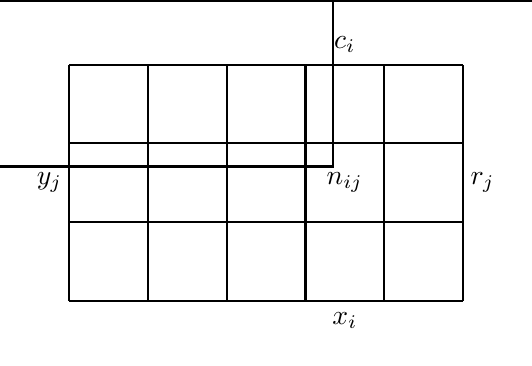
\begin{tikzpicture}
\draw [step=1.0, black, thick] (0, 0) grid (5, 3);
\node at (3.5, 3.25) {$c_i$};
\node at (5.25, 1.5) {$r_j$};
\node at (3.5, -0.25) {$x_i$};
\node at (-0.25, 1.5) {$y_j$};
\node at (3.5, 1.5) {$n_{ij}$};
\end{tikzpicture}
\end{center}

joint probability of $X = x_i$ and $Y = y_j$ :

\begin{equation}
p(X = x_i, Y = y_j) = \frac{n_{ij}}{N}
\tag{1.5}
\end{equation}

\begin{description}[labelwidth=\widthof{\bfseries 1234567890},align=parright]
	\item[$X = x_i :$] probability $X$ take value $x_i$
	\item[$Y = y_j :$] probability $Y$ take value $y_j$
\end{description}


\bigskip



\begin{equation}
\tag{}
\end{equation}

\begin{description}[labelwidth=\widthof{\bfseries 1234567890},align=parright]
	\item[$!$] !
	\item[$!$] !
\end{description}


\end{document}